\documentclass[conference]{IEEEtran}
\IEEEoverridecommandlockouts
% The preceding line is only needed to identify funding in the first footnote. If that is unneeded, please comment it out.
\usepackage{cite}
\usepackage{amsmath,amssymb,amsfonts}
\usepackage{algorithmic}
\usepackage{graphicx}
\usepackage{textcomp}
\usepackage{xcolor}
\usepackage[spanish]{babel}

\def\BibTeX{{\rm B\kern-.05em{\sc i\kern-.025em b}\kern-.08em
    T\kern-.1667em\lower.7ex\hbox{E}\kern-.125emX}}
\begin{document}

\title{Trabajo Práctico "Disipadores"\\
{\footnotesize \textsuperscript{}Curso 2023 - Tecnología de los Materiales Electrónicos}
\thanks{}
}

\author{\IEEEauthorblockN{1\textsuperscript{st} Ramiro Belsito}
\IEEEauthorblockA{\textit{Estudiante} \\
\textit{Instituto Tecnológico de Buenos Aires}\\
Buenos Aires, Argentina\\
rabelsito@itba.edu.ar}
\and
\IEEEauthorblockN{2\textsuperscript{nd} Facundo Caviglia}
\IEEEauthorblockA{\textit{Estudiante} \\
\textit{Instituto Tecnológico de Buenos Aires}\\
Buenos Aires, Argentina \\
fcaviglia@itba.edu.ar}}

\maketitle


\begin{abstract}
En el siguiente informe se analizará la utilidad de dos disipadores proveídos por la cátedra
para el buen funcionamiento de un regulador de tensión con encapsulado TO220.
\end{abstract}

\section{Introduction}
Se analizará la resistencia térmica de estos por medio de la práctica y se comparará con los valores 
obtenidos por medio de las ecuaciones teóricas y la hoja de datos del fabricante. Con estos datos
se realizará el circuito térmico equivalente y se intentará realizar simulaciones para poder contrastar
los resultados obtenidos empíricamente. Además se estudiará la influencia del posicionamiento del disipador,
frente a la posición óptima.

\section{Forma y Dimensiones}
\begin{figure}[h]
    \centering
    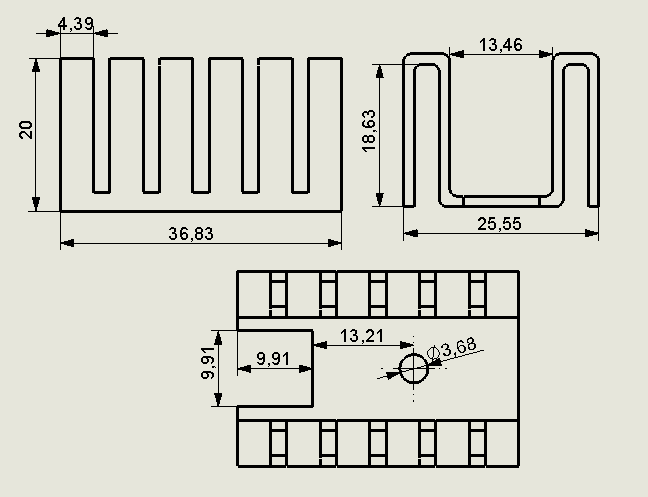
\includegraphics[width=0.3\textwidth]{PlanoRamiCompleto.png}
    \caption{Plano del disipador 1}
    \centering
    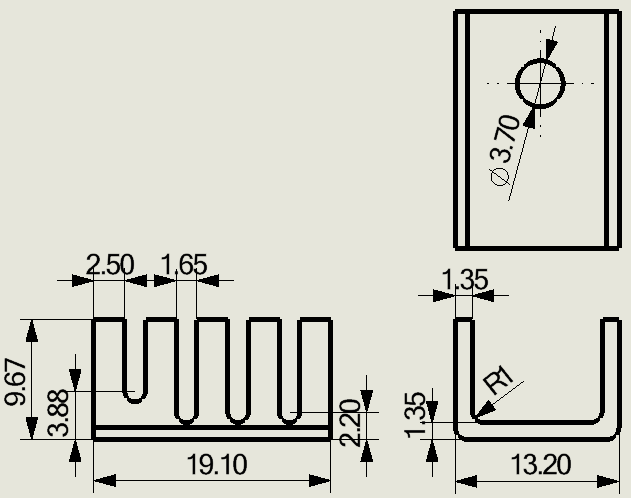
\includegraphics[width=0.3\textwidth]{disipadorFacu.png}
    \caption{Plano del disipador 2}
\end{figure}
Ambos disipadores son estampados sobre una plancha de aluminio anodizado, y luego tratado con otros 
procesos mecánicos para obtener la forma de cada uno. Por su método de fabricación cada disipador
es una pieza única, a diferencia de los fabricados por extrusión, que son piezas continuas cortadas 
a la medida requerida

\section{Cálculos Teóricos}
\subsection{Disipador 1}

La superficie de contacto, obtenida a través del modelado en Solidworks, es de 6915,40$mm^2$ y
su distancia vertical ($d_v$) es de 25,55$mm$.
Por lo tanto, mediante la ecuación de la resistencia térmica por convección natural se obtiene:
\begin{equation}
    R_{sa} = \frac{1}{1,34\cdot A_s}\cdot (\frac{d_v}{\Delta T})^{\frac{1}{4}} = \frac{1}{1,34\cdot 6915,40mm^2}\cdot (\frac{25,55mm}{150-25})^{\frac{1}{4}}
\end{equation}

\section{Mediciones Experimentales}
A continuación pueden observarse las mediciones llevadas a cabo en el laboratorio. Se analizaron
distintas posiciones para cada disipador y se concluirá su posición más eficiente para la convección
natural. Se estudiará la corriente en la salida del LM317 y su tensión, así teniendo idea de la potencia
que está disipando el componente. Además, se analiza el comportamiento del disipador con la presencia 
de grasa siliconada.

\begin{table}[htbp]
    \caption{Mediciones sobre los Disipadores}
    \begin{center}
    \begin{tabular}{|c|c|c|c|}
    \hline
    \textbf{Mediciones} & \multicolumn{3}{|c|}{\textbf{Número de Disipador}} \\
    \cline{2-4} 
    \textbf{de Laboratorio} & \textbf{\textit{Sin Disipador}} & \textbf{\textit{Disipador 1}} & \textbf{\textit{Disipador 2}} \\
    \hline
    $I_{m\acute{i}n}$ (sin grasa) & 0,21A & 0,9A & 0,45A \\
    \hline
    $I_{m\acute{i}x}$ (con grasa) & - & 1,11A & 0,52A \\
    \hline
    $V$ & 12v & 11,96v & 12v \\
    \hline
    $Q$ (sin grasa) & 2,52W & 10,76W & 5,4W \\
    \hline
    $Q$ (con grasa) & - & 13,28W & 6,24W \\
    \hline
    \end{tabular}
    \label{tab1}
    \end{center}
    \end{table}

    \begin{table}[htbp]
        \caption{Diferencias entre las posiciones del Disipador}
        \begin{center}
        \begin{tabular}{|c|c|c|}
        \hline
        \textbf{Mediciones} & \multicolumn{2}{c|}{\textbf{Número de Disipador}} \\
        \cline{2-3}
        \textbf{de Laboratorio} & \textbf{\textit{Disipador 1}} & \textbf{\textit{Disipador 2}} \\
        \hline
        $I_{m\acute{i}n}$ (posicion 1) & 0,9A & 0,45A \\
        \hline
        $I_{m\acute{i}n}$ (posicion 2) & 0,82A & 0,43A \\
        \hline
        $I_{m\acute{i}n}$ (posicion 3) & 0,85A & 0,44A \\
        \hline
        
        \end{tabular}
        \label{tab1}
        \end{center}
    \end{table}

\end{document}
